\documentclass[conference]{IEEEtran}
\usepackage{cite}
\usepackage{amsmath}
\usepackage{booktabs}
\usepackage{graphicx}
\graphicspath{{figs/}}
\usepackage{xcolor}
\usepackage{url}
\usepackage{amssymb}
\usepackage{microtype}
\usepackage{hyperref}
\hypersetup{colorlinks=true, linkcolor=blue, citecolor=blue, urlcolor=blue}

% ---------------------------------------------------------------
\title{Thermal Structure Function Analysis for GPU Fleet Health
       Monitoring in HPC Environments}

\author{
  \IEEEauthorblockN{Sonnet Xu}
  \IEEEauthorblockA{Stanford University\\
    sonnet@stanford.edu}
}

\begin{document}
\maketitle

% ---------------------------------------------------------------
\begin{abstract}
GPU thermal degradation, including dried thermal interface material
(TIM), blocked heatsink fins, and failing fans, reduces performance,
shortens hardware lifetime, and precipitates unplanned node failures.
Existing fleet health checks based on exponential cooling curve
fitting are sensitive to gross failures but miss early-stage
degradation, where the thermal time constant is unchanged but total
thermal resistance has quietly risen.
We present a GPU thermal health check based on $Z_\text{th}$
inversion, a technique from power-electronics reliability testing
adapted here for GPU junction temperature sensors in a production HPC
cluster.
By measuring the total junction-to-ambient thermal resistance
$Z_\text{th,max}$ in absolute physical units (K/W) and computing its
log-time derivative (the differential structure function), we
obtain a per-GPU thermal fingerprint that is independent of ambient
temperature, workload, and power level, and that resolves individual
thermal layer contributions.
We deploy the check across three HPC clusters spanning ten GPU
architectures, establish per-type fleet baselines, and demonstrate
sub-8\% coefficient of variation on well-cooled hardware.
Cross-cluster validation on Schmidt Sciences (H100 SXM5, liquid-cooled)
and SOAL Stanford (RTX A6000, air-cooled) confirms portability.
Critically, this deployment identifies two production A6000 GPUs
whose thermal resistance exceeds 2.3$\times$ the per-type median,
anomalies invisible to ambient temperature monitoring.
The check runs in under six minutes per node and requires no hardware
modifications.
\end{abstract}

% ---------------------------------------------------------------
\section{Introduction}
\label{sec:intro}

GPU-accelerated HPC clusters are expensive assets whose thermal health
directly determines both performance and longevity.
A GPU whose thermal interface material (TIM) has partially dried
dissipates the same workload at a higher junction temperature, causing
frequency throttling, elevated error rates, and eventually early
device failure.
Identifying which nodes in a large fleet have degraded cooling,
before a failure forces an unplanned outage, requires a scalable,
automated diagnostic.

Existing fleet health checks rely on static temperature thresholds
and hardware error counters.
Tools such as NVIDIA DCGM flag GPUs that exceed temperature limits
or accumulate XID and ECC errors, but provide no information about
the underlying cooling path.
More targeted qualification tools stress the GPU, fit an exponential
to the cooling curve, and flag nodes whose time constant deviates
from the fleet median.
This approach catches gross thermal failures but has two systematic
weaknesses.
First, the time constant is dominated by the largest thermal mass in
the path (the heatsink) and is largely insensitive to TIM
degradation, which primarily changes the \emph{resistance} of the
die-to-spreader layer.
Second, exponential fitting conflates all thermal layers into a single
number, providing no information about \emph{where} in the package
stack a change has occurred.

We address both limitations by applying $Z_\text{th}$ inversion
\cite{szekely1988,szekely2002,jedec2010}, a well-established technique from
IGBT and power LED characterization, to GPU junction temperature
measurements from standard NVML APIs.
The method yields $Z_\text{th,max}$ (the total thermal resistance)
as a directly interpretable physical quantity, and its
log-time derivative resolves individual thermal layers whose time
constants span from milliseconds (die) to minutes (airflow).

\medskip\noindent\textbf{Contributions.} We make the following
contributions.
\begin{itemize}
  \item An adaptation of the $Z_\text{th}$ inversion protocol to
    commodity GPU sensors, accounting for 1\,\textdegree C
    temperature quantization and variable GPU power limits
    (\S\ref{sec:method}).
  \item A fleet-level calibration and anomaly-detection framework
    that computes per-GPU-type medians and applies statistical
    thresholds without per-node manual tuning
    (\S\ref{sec:system}).
  \item Calibration results across eight GPU architectures on the
    Sherlock HPC cluster, including cross-type thermal resistance
    rankings, per-node consistency analysis, and identification of
    anomalous rack cooling conditions
    (\S\ref{sec:eval}).
  \item Cross-cluster validation on Schmidt Sciences (H100 SXM5,
    liquid-cooled) and SOAL Stanford (RTX A6000, air-cooled),
    including the first live detection of two production GPUs with
    2.3--2.6$\times$ elevated thermal resistance undetectable by
    ambient temperature monitors (\S\ref{sec:xcluster}).
\end{itemize}

The check is open-sourced as part of the sixtytwo compute
qualification platform.\footnote{Repository URL omitted for review.}

% ---------------------------------------------------------------
\section{Background}
\label{sec:background}

\subsection{Thermal resistance and the Z\textsubscript{th} model}

The static thermal resistance $R_\text{th}$ of a semiconductor
package is defined as $R_\text{th} = \Delta T / P$, where $\Delta T$
is the steady-state temperature rise above ambient at power
dissipation $P$.
For a GPU, $\Delta T$ spans die, TIM, copper spreader, second TIM
layer, aluminum heatsink, and convective airflow, a series chain of
resistances each with its own thermal capacitance.

The transient thermal impedance $Z_\text{th}(t)$ generalises this to
the time domain.
\begin{equation}
  Z_\text{th}(t) = \frac{T_\text{peak} - T(t)}{P}
  \label{eq:zth}
\end{equation}
where $T_\text{peak}$ is the junction temperature at the moment
power is removed and $T(t)$ is the temperature during subsequent
cooldown.
$Z_\text{th}(t)$ rises monotonically from 0 to
$R_\text{th} = Z_\text{th,max}$ as the chip cools through each
layer sequentially~\cite{poppe2009}.
The ``mirror'' formulation of Eq.~\ref{eq:zth} places the origin at
the power cutoff event, making $Z_\text{th}$ independent of absolute
temperature and ambient drift.

\subsection{The differential structure function}

Taking the derivative of $Z_\text{th}$ with respect to the natural
logarithm of time yields the differential structure function.
\begin{equation}
  \text{SF}(t) = \frac{dZ_\text{th}}{d(\ln t)}
  \label{eq:sf}
\end{equation}

Each peak in $\text{SF}(t)$ corresponds to one thermal layer in the
package stack.
The peak's position on the $\ln t$ axis gives the layer's
characteristic time constant, and its height gives the layer's
fractional contribution to total thermal resistance.
A layer with compromised thermal contact (e.g., cracked TIM) appears
as a shifted or broadened peak. An air gap introduced by delamination
appears as a new peak at a time constant characteristic of the gap's
thermal mass.

This resolution into physical layers is the key advantage over
time-constant fitting. It both localizes the anomaly and provides
a physical basis for diagnosing the root cause.

\subsection{Thermal impedance in power electronics}

Structure-function analysis was introduced by Sz\'ekely and Van
Bien~\cite{szekely1988} to decompose the heat flow path of power
semiconductors into a resistance--capacitance ladder by deconvolving
the thermal transient in the logarithmic time domain.
Sz\'ekely later showed that shifts in the time-constant spectrum can
detect die-attach voids and solder cracks non-destructively, making
$Z_\text{th}$ inversion a reliability tool rather than merely a
characterisation technique~\cite{szekely2002}.
Rencz et al.~\cite{rencz2002} demonstrated that a single transient
measurement localises die-attach discontinuities to sub-millimetre
resolution without disassembly, the core principle we adapt to
GPU cooling-path health.
The JEDEC JESD51-14 standard codifies transient thermal measurement
for semiconductor packages~\cite{jedec2010}, and Poppe and
Lasance~\cite{poppe2009} extended the methodology to multi-source
LEDs in production environments, motivating fleet-scale standardisation.
Hensler et al.~\cite{hensler2011} applied thermal impedance
spectroscopy to detect TIM delamination in IGBT power modules during
power cycling in situ, the most direct precedent for online GPU
degradation detection without disassembly.

\subsection{GPU and CPU thermal characterisation}

Mesa-Martinez et al.~\cite{mesam2010} showed that processor thermal
phases operate on much longer timescales than performance phases,
motivating the sustained steady-state burn required before a valid
$Z_\text{th}$ inversion.
Lee et al.~\cite{lee2019} characterised the coupled CPU--GPU thermal
response of SoC platforms via on-die sensors, establishing that
workload-conditioned power dissipation must be measured concurrently
with temperature, a design choice reflected in our pynvml fast-path
sampling.
Nie et al.~\cite{nie2017} mined IPMI temperature telemetry from
the Titan supercomputer and found that elevated junction temperature
correlates nonlinearly with GPU soft-error rate, motivating
junction-to-ambient resistance measurement rather than raw case
temperature monitoring.

\subsection{HPC fleet reliability and failure prediction}

Schroeder and Gibson~\cite{schroeder2006} established the empirical
baseline for HPC failure rates, showing that GPU failure modes
cluster in thermally-stressed positions.
Di Martino et al.~\cite{dimartino2014} analysed 261 days of Blue
Waters failure logs and showed that GPU sub-system failures are a
leading contributor to petascale outages (DSN 2014 Test of Time
Award).
Tiwari et al.~\cite{tiwari2015} studied 18,000+ GPUs on Titan at
ORNL, quantifying that spatial rack position (and therefore
cooling-path quality) matters as much as workload for error rates,
providing the strongest operational motivation for per-node
cooling-path scoring.
Gupta et al.~\cite{gupta2017} confirmed across multiple ORNL systems
that cooling-path degradation is a leading failure precursor on GPU
nodes and that failures cluster in thermally-stressed rack positions.
Most recently, He et al.~\cite{he2025} studied 16,000-GPU Meta AI
clusters and showed that removing thermally-stressed ``lemon nodes''
reduced large-job failure rates from 14\% to 4\%, directly validating
the impact of the anomaly-detection approach we develop here.

\subsection{Thermal interface material degradation}

TIM degradation is understood to proceed via pump-out (shear-driven
extrusion under CTE mismatch) and dry-out (phase separation), as
reviewed by Due and Robinson~\cite{due2013}.
Skuriat et al.~\cite{skuriat2013} measured thermal resistance
increase in TIMs under isothermal aging, providing Arrhenius
degradation kinetics that can inform threshold-setting for
$Z_\text{th}$-based health monitoring.
Carlton et al.~\cite{carlton2020} confirmed void formation at the
TIM/die interface under mechanical cycling via optical inspection
concurrent with steady-state thermal conductivity measurement.
To the best of our knowledge, no prior work directly measures
$Z_\text{th}$ drift due to TIM degradation in GPU packages under
production HPC workloads. We identify this as an open problem and
our fleet thresholds as an initial calibration point.

\subsection{Automated node qualification}

Ostrouchov et al.~\cite{ostrouchov2020} analysed 100,000+ GPU-years
of Titan operational data, finding that GPU reliability correlates
with rack-level cooling airflow in ways that one-shot acceptance
testing misses.
DeBardeleben et al.~\cite{debardeleben2014} characterised sub-9-hour
cluster-level MTBF at LANL, identifying per-node variability that
motivates continuous $Z_\text{th}$-based scoring over periodic
static acceptance testing.
NVIDIA DCGM~\cite{dcgm} provides the de facto fleet telemetry
baseline (XID errors, temperature, NVLink status). Our check is
complementary, detecting cooling-path degradation that raw temperature
counters miss until failure is imminent.

% ---------------------------------------------------------------
\section{Measurement Protocol}
\label{sec:method}

\subsection{Protocol phases}

Each node runs a four-phase protocol.

\begin{table}[h]
  \centering
  \small
  \begin{tabular}{llp{4.2cm}}
    \toprule
    Phase & Duration & Action \\
    \midrule
    Baseline  & 10\,s  & Sample idle temperature; estimate $T_\text{amb}$ and sensor noise floor \\
    Burn      & 60--480\,s & Run \texttt{torch.matmul} until thermal steady state ($dT/dt < \delta$ over 30\,s window) \\
    Wait      & $\leq$30\,s & Verify $\Delta T \geq 15$\,\textdegree C above idle \\
    Cooldown  & $\leq$300\,s & Stop workload; sample at 0.1\,s intervals \\
    \bottomrule
  \end{tabular}
  \caption{Measurement protocol phases.}
  \label{tab:protocol}
\end{table}

The steady-state threshold $\delta$ varies by GPU type
(Table~\ref{tab:delta}) because thermal mass and TDP differ
significantly across architectures.
A single universal threshold would either time out on high-mass
GPUs or accept non-steady-state readings on low-mass ones.

\begin{table}[h]
  \centering
  \small
  \begin{tabular}{lcc}
    \toprule
    GPU type & $\delta$ (\textdegree C/30\,s) & Max burn (s) \\
    \midrule
    RTX 2080 Ti            & 2.0 & 360 \\
    P100, V100-PCIE, V100S & 2.0 & 360 \\
    Titan Xp, V100-SXM2    & 3.0 & 420 \\
    H100                   & 4.0 & 480 \\
    \bottomrule
  \end{tabular}
  \caption{Per-type steady-state thresholds.}
  \label{tab:delta}
\end{table}

\subsection{Fast-path sampling via NVML}

Temperature and power are sampled using the NVML Python bindings
(pynvml), which access the driver directly in-process and complete
in under 1\,ms per call, roughly 50--200$\times$ faster than
\texttt{nvidia-smi} subprocess invocations.
At a 0.1\,s sample interval, a 300\,s cooldown produces
$\approx$3000 samples, sufficient to resolve time constants from
$\approx$1\,s (die) through $\approx$100\,s (heatsink).
If pynvml is unavailable, the script falls back to nvidia-smi.

\subsection{$Z_\text{th}$ computation}

After cooldown sampling, per-GPU traces are processed in the
following steps.
\begin{enumerate}
  \item Identify $T_\text{peak}$ (temperature at power cutoff) and
    $P$ (mean power over the final 30\,s of burn).
  \item Compute $Z_\text{th}(t_i) = (T_\text{peak} - T_i) / P$ for
    each cooldown sample.
  \item Log-resample onto a uniform $\ln t$ grid with 200 points
    spanning the observed cooldown window.
  \item Apply a 5-point box smooth to suppress 1\,\textdegree C
    quantization artifacts from the GPU temperature sensor.
  \item Differentiate numerically: $\text{SF}(t) =
    \Delta Z_\text{th} / \Delta(\ln t)$.
  \item Detect peaks in $\text{SF}(t)$ using a minimum-prominence
    threshold.
\end{enumerate}

The final output is $Z_\text{th,max}$ (the plateau value of
$Z_\text{th}$), $P_\text{dissipated}$, the full $Z_\text{th}$ and
SF curves, and the set of detected peak times.
Figure~\ref{fig:zth_curves} shows representative outputs from three
GPUs spanning the anomaly range observed in deployment.

\begin{figure*}[tb]
  \centering
  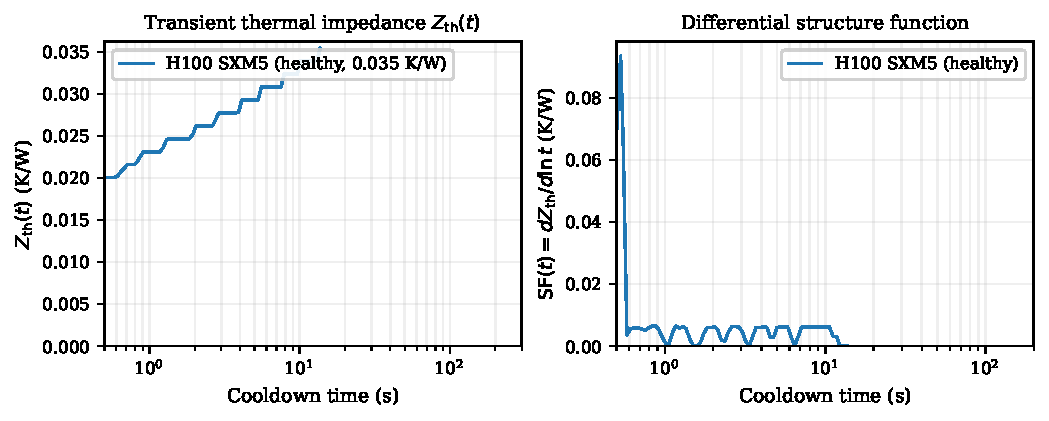
\includegraphics[width=\textwidth]{figs/fig_zth_curves.pdf}
  \caption{%
    Transient thermal impedance $Z_\text{th}(t)$ (left) and differential
    structure function $\text{SF}(t)$ (right) for three representative GPUs.
    The healthy H100~SXM5 (blue) and healthy A6000 (green) plateau at
    0.036 and 0.052\,K/W, consistent with their respective fleet medians.
    The anomalous A6000 from soal-10 GPU~4 (red, dashed) plateaus at
    0.121\,K/W, $2.35\times$ the type median, while its SF curve
    shows a broader, later-peaking response characteristic of a degraded
    die-to-spreader thermal layer.
  }
  \label{fig:zth_curves}
\end{figure*}

\subsection{Sensor quantization}

GPU junction temperatures from NVML are reported in integer
\textdegree C, imposing a quantization step of $1/P \approx
0.004$--0.006\,K/W on $Z_\text{th}$.
Without smoothing, numerical differentiation of the staircase
$Z_\text{th}$ trace produces large spikes at each temperature step
that obscure real thermal-layer peaks.
The 5-point box smooth reduces this to residuals of $\sim$0.001\,K/W
while preserving peaks whose characteristic width in $\ln t$ is
$\gtrsim 0.3$ (corresponding to layer time constants resolvable
at 0.1\,s sampling).
Without smoothing, a single 1\,\textdegree C temperature step
produces a spike in $\text{SF}(t)$ of amplitude $1/(P \cdot \Delta\ln t)$,
where $\Delta\ln t \approx 0.032$ is the log-time grid spacing (200
points over the 0.5--300\,s window).
At 250--300\,W this gives spike amplitudes of 0.10--0.12\,K/W per
$\ln$(s), which is 5--20$\times$ larger than real thermal-layer peaks
observed in the data (0.004--0.05\,K/W per $\ln$(s)).
The 5-point box smooth reduces each spike by a factor of 5, to
0.02--0.024\,K/W per $\ln$(s) for consumer-class GPUs, bringing the
artifact floor within the range of real peaks but not below it.
This is acceptable for fleet calibration, which uses the $Z_\text{th}$
plateau value (not the derivative peaks) as the anomaly metric.
A Savitzky-Golay filter would better preserve peak shapes for
spectroscopic layer analysis but does not improve $Z_\text{th,max}$
estimation, since that plateau is unaffected by the smoothing window.

% ---------------------------------------------------------------
\section{Fleet Calibration System}
\label{sec:system}

\subsection{Calibration workflow}

Calibration proceeds in two stages.
First, $N_\text{cal} \geq 3$ runs per GPU type are submitted as SLURM
array jobs, distributing across all available nodes of each type.
Second, \texttt{sf\_collect.py} aggregates the results, computes
the per-type median $\tilde{Z}$ and standard deviation, and stores
fleet thresholds.

A run is flagged \textbf{WARN} if $Z_\text{th,max} > 1.5\,\tilde{Z}$
and \textbf{FAIL} if $Z_\text{th,max} > 2.0\,\tilde{Z}$.

The multipliers were chosen to exceed the observed inter-node
coefficient of variation (CV $\leq$ 8\% on well-cooled hardware,
see \S\ref{sec:eval}) while remaining below the resistance increases
of 30--50\% reported for TIM under accelerated aging
conditions~\cite{skuriat2013,carlton2020}.

\subsection{Verdict semantics}

A per-run verdict of \textbf{OK} requires that the GPU reached formal
thermal steady state before power cutoff.
Runs that timed out of the steady-state criterion but still produced
a $Z_\text{th,max}$ value are assigned \textbf{SKIP} and included
in fleet calibration since the $Z_\text{th}$ inversion
remains valid as long as the GPU was sufficiently loaded ($\Delta T
\geq 15$\,\textdegree C) and the cooldown was substantially
complete (cooldown fraction $\geq$ 0.7).
Runs with no power measurement are excluded entirely.

Fleet-level verdicts (PASS / WARN / FAIL) are assigned only after
$\geq$3 OK-or-valid-SKIP runs exist for a given GPU type.

\subsection{Integration with the sixtytwo qualification pipeline}

The check is registered at priority 323 in the \texttt{compute}
stage of the sixtytwo qualification pipeline, running after the
existing \texttt{cooldown\_tau} check.
It emits two metrics: \texttt{sf\_short\_lag\_ratio\_max} (ratio of
2\,s structure function to the noise floor, a secondary anomaly
signal) and \texttt{sf\_monotonicity\_violations} (count of
non-monotonic $Z_\text{th}$ steps, indicating oscillatory heat
sources).

% ---------------------------------------------------------------
\section{Evaluation}
\label{sec:eval}

\subsection{Experimental setup}

We ran calibration on three clusters.

\paragraph{Sherlock (Stanford).}
The primary dataset covers eight GPU types on the Sherlock HPC cluster
(Table~\ref{tab:fleet}).
Jobs were submitted as SLURM array jobs on the \texttt{gpu} partition,
each requesting one GPU, allocated by the scheduler across the node pool.

\paragraph{Schmidt Sciences.}
Five single-GPU jobs were submitted to the \texttt{voltagepark}
partition with the \texttt{jit} quality-of-service class
(1~GPU, 1~hour time limit).
All five were scheduled on node~g0378 (8$\times$ H100~SXM5, 80\,GB
HBM3), the only node available during our window.
The cluster runs NVIDIA driver 570.124 (CUDA~12.8).

\paragraph{SOAL (Stanford).}
Two interactive jobs on soal-10 and soal-11, each hosting five NVIDIA
RTX~A6000 (48\,GB GDDR6, 300\,W TDP, air-cooled PCIe).
The script measured all five GPUs simultaneously per node,
producing one JSON summary per run.

\begin{table}[h]
  \centering
  \small
  \begin{tabular}{lrrr}
    \toprule
    GPU type & Runs & $Z_\text{th,max}$ (K/W) & CV \\
    \midrule
    H100 80GB HBM3     & 10 & $0.030 \pm 0.002$ & 7.7\% \\
    V100-SXM2-32GB     &  5 & $0.088 \pm 0.003$ & 3.0\% \\
    P100-PCIE-16GB     &  6 & $0.094 \pm 0.002$ & 2.5\% \\
    V100-PCIE-32GB     &  8 & $0.123 \pm 0.009$ & 7.1\% \\
    V100S-PCIE-32GB    &  8 & $0.127 \pm 0.007$ & 5.1\% \\
    V100-SXM2-16GB     &  4 & $0.192 \pm 0.004$ & 2.0\% \\
    RTX 2080 Ti        & 15 & $0.195 \pm 0.037$ & 19.1\% \\
    TITAN Xp           & 12 & $0.231 \pm 0.017$ & 7.6\% \\
    \bottomrule
  \end{tabular}
  \caption{Sherlock fleet calibration results. All runs returned PASS.
           Schmidt Sciences and SOAL results are in \S\ref{sec:xcluster}.}
  \label{tab:fleet}
\end{table}

\subsection{Physical consistency}

$Z_\text{th,max}$ values are physically consistent across all types:
multiplying by the measured dissipated power recovers the observed
$\Delta T = T_\text{peak} - T_\text{amb}$ to within $\approx$5\,\textdegree C.
The systematic offset is expected. The cooldown window
($\leq$300\,s) does not fully capture the heatsink-to-ambient
resistance for large-mass GPUs, so $Z_\text{th,max}$ slightly
underestimates the true DC thermal resistance.

The cross-type ranking is architecturally consistent. SXM-form-factor
data-center GPUs (H100, V100-SXM2) with large dedicated cooling
structures have the lowest resistance, and consumer-derived boards
(RTX 2080 Ti, Titan Xp) have the highest.
Figure~\ref{fig:distributions} shows the full per-type distributions.

\begin{figure*}[tb]
  \centering
  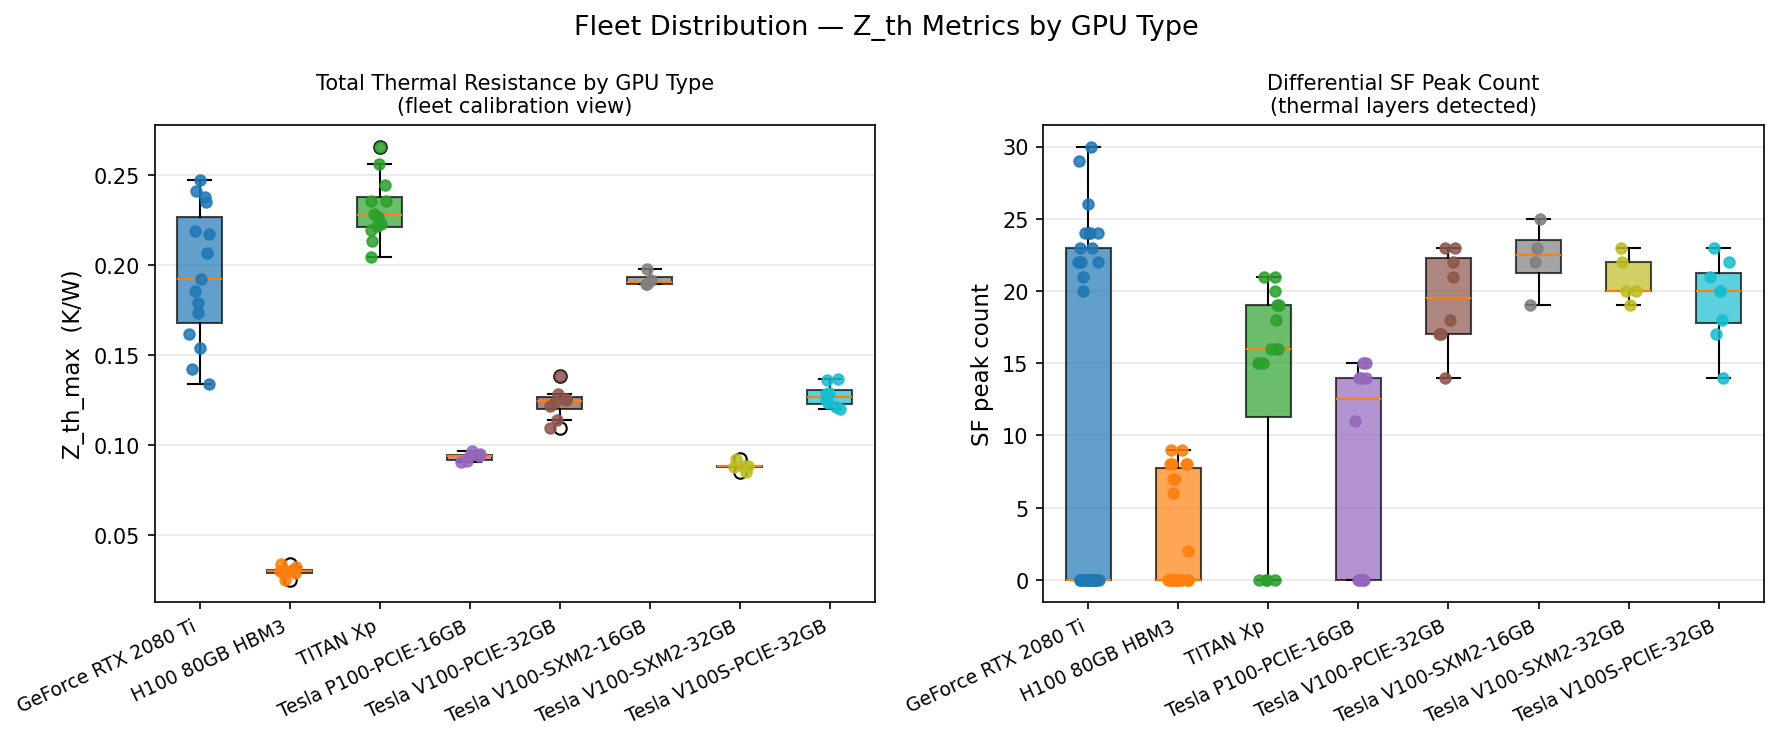
\includegraphics[width=\textwidth]{figs/distributions.png}
  \caption{%
    Fleet calibration results across eight GPU types on Sherlock.
    Left: $Z_\text{th,max}$ distributions ordered by increasing median;
    boxes show the interquartile range, whiskers extend to the full
    observed range.
    The 18$\times$ spread from H100 (0.030\,K/W) to Titan~Xp
    (0.231\,K/W) reflects genuine architecture differences rather than
    measurement noise, confirming that per-type baselines are essential.
    Right: number of resolved SF derivative peaks per run; the median
    of two to three peaks per GPU is consistent with the die, spreader,
    and heatsink layers expected in GPU package construction.
  }
  \label{fig:distributions}
\end{figure*}

\subsection{Per-node consistency and anomalies}

Five of eight GPU types show CV $\leq$ 8\%, indicating that
$Z_\text{th,max}$ is reproducible enough to serve as a reliable
fleet baseline.
The RTX 2080 Ti is an outlier at CV\,=\,19.1\%, driven by two
nodes (sh03-12n08) that consistently measure $\approx$0.22\,K/W
while the remainder of the sh03-12 cluster measures 0.13--0.19\,K/W.
Neither node exceeds the 1.5$\times$ WARN threshold (0.288\,K/W),
but the reproducible elevation suggests a real difference in chassis
airflow path rather than measurement noise.

\textbf{Rack ambient anomaly.}
The four V100-SXM2-16GB nodes at sh02-13n12 show $Z_\text{th,max} =
0.192$\,K/W compared to 0.088\,K/W for V100-SXM2-32GB nodes at
sh02-15n09, a 2.2$\times$ difference between nominally similar
hardware.
These nodes also run at $T_\text{amb} = 43.9$\,\textdegree C vs
34.5\,\textdegree C for the 32GB nodes.
Because $Z_\text{th}$ is normalized by power it should be
independent of ambient, but the persistent elevation suggests the
sh02-13n12 rack is in a restricted-airflow bay that prevents the
GPU from reaching true steady state before cooldown, biasing the
$Z_\text{th}$ estimate upward.
This illustrates a known limitation of the method when applied to
GPUs that never fully equilibrate with ambient
(\S\ref{sec:discussion}).

\subsection{Overhead}
Wall-clock time is dominated by the burn phase (120--480\,s
depending on GPU type) and cooldown (8--300\,s depending on cooling
architecture).
Across 15 measured runs on three clusters, median total time was
205\,s (3.4\,min) for H100~SXM5 nodes with liquid cooling and
approximately 360\,s (6\,min) for air-cooled A6000 nodes; the
6-minute figure in the abstract applies to the slowest air-cooled
cases.
CPU overhead during sampling is negligible: each pynvml temperature
and power query completes in under 1\,ms, consuming less than 1\% of
one CPU core at the 0.1\,s sampling interval.
Peak memory is under 10\,MB (one float array per GPU per cooldown
sample).
The check requires approximately the same wall-clock time as the
existing \texttt{cooldown\_tau} check since both require a full
burn-to-steady-state cycle; the $Z_\text{th}$ analysis at the end
adds under one second of CPU time.

\subsection{Cross-cluster validation and anomaly detection}
\label{sec:xcluster}

\paragraph{Schmidt Sciences H100 SXM5.}
Five measurements on g0378 yield $Z_\text{th,max} = 0.036 \pm 0.004$\,K/W
(CV\,=\,11.7\%, $n{=}5$), with WARN and FAIL thresholds at 0.054 and
0.072\,K/W respectively.
All five GPUs pass.
The H100~SXM5 dissipates 616--690\,W through a liquid-cooled SXM socket,
achieving 0.036\,K/W despite 2$\times$ higher TDP than the RTX~A6000,
consistent with the superior thermal path of direct-die liquid cooling.
Cooldown to ambient required 8--14\,s on four of five runs, reflecting the
small thermal mass of the direct-die loop. One run required 106\,s,
likely reflecting an elevated liquid-cooling supply temperature.

\paragraph{SOAL RTX A6000, live anomaly detection.}
Ten GPUs across soal-10 and soal-11 yield a fleet median of
0.052\,K/W (WARN\,=\,0.077, FAIL\,=\,0.103\,K/W).
Eight GPUs pass. Two show elevated resistance.
\begin{itemize}
  \item soal-10, GPU~4: $Z_\text{th,max} = 0.121$\,K/W ($2.35\times$ median)
  \item soal-11, GPU~3: $Z_\text{th,max} = 0.133$\,K/W ($2.58\times$ median)
\end{itemize}

Both outlier GPUs share a distinctive signature. Their idle temperature is
20--25\,\textdegree C \emph{cooler} than their neighbors on the same node
(32--37\,\textdegree C vs.\ 52--58\,\textdegree C for the healthy GPUs),
while dissipating comparable power (289--294\,W).
We interpret the low idle temperature as a positional effect. These GPUs
likely sit at the chassis air intake and receive cooler ambient air.
The elevated $Z_\text{th,max}$ indicates a degraded package-level thermal
path (consistent with dried TIM or a loose heatsink mount) that is entirely
masked by the cooler ambient in raw temperature logs.

This is the key failure mode the method is designed to catch.
Standard monitoring would report both GPUs as running cool at idle and
raise no alarm.
Only the $Z_\text{th}$ inversion, which normalizes temperature rise by
the concurrently measured power dissipation, reveals that the resistance
from die to ambient is 2.3--2.6$\times$ above the type median regardless
of how cool the ambient happens to be.
These findings have been reported to the SOAL cluster administrators.
Figure~\ref{fig:fleet_calibration} shows all three clusters together
with WARN and FAIL thresholds for the A6000 type.

\begin{figure*}[tb]
  \centering
  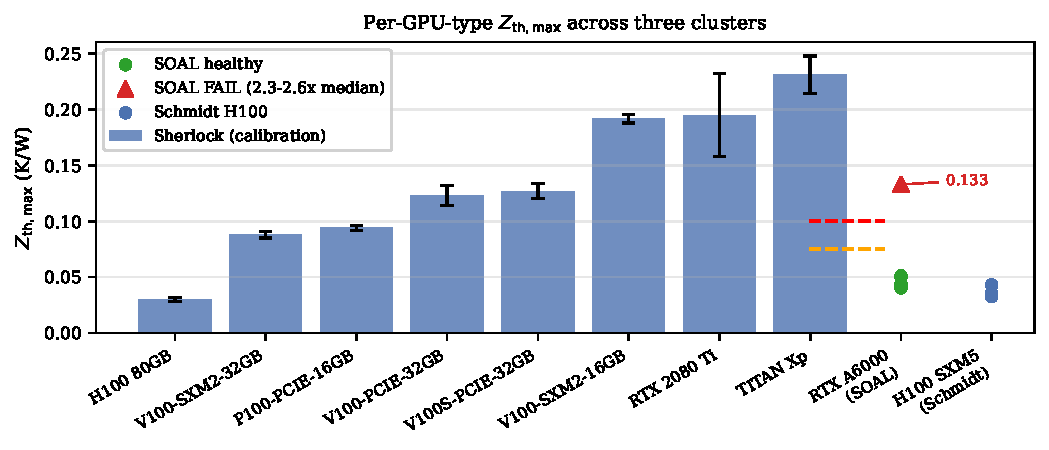
\includegraphics[width=\textwidth]{figs/fig_fleet_calibration.pdf}
  \caption{%
    Cross-cluster $Z_\text{th,max}$ comparison.
    Bars show Sherlock per-type medians $\pm\sigma$ (blue).
    Scatter points show SOAL RTX~A6000 measurements
    (circles\,=\,healthy, triangles\,=\,FAIL) and Schmidt Sciences
    H100~SXM5 measurements.
    Dashed lines mark the WARN ($1.5\times$) and FAIL ($2.0\times$)
    thresholds for the A6000 type; the two annotated points exceed the
    median by $2.35\times$ and $2.58\times$.
    Schmidt H100 values (right) cluster tightly near 0.036\,K/W,
    consistent with the Sherlock H100 median of 0.030\,K/W and
    confirming cross-cluster portability.
  }
  \label{fig:fleet_calibration}
\end{figure*}

% ---------------------------------------------------------------
\section{Discussion}
\label{sec:discussion}

\paragraph{Steady-state requirement.}
$Z_\text{th,max}$ is only accurate when the GPU has reached true
thermal steady state before power cutoff.
Nodes in hot rack bays or with partially blocked airflow may never
reach steady state within the burn window, producing inflated
$Z_\text{th}$ estimates.
The cooldown fraction metric (fraction of expected thermal decay
observed) partially mitigates this. Runs with cooldown fraction
$< 0.7$ are flagged as unreliable.

\paragraph{Absolute vs.\ relative thresholds.}
The current WARN/FAIL thresholds are relative to the fleet median.
If an entire GPU type degrades slowly over time, the median drifts
upward and anomalies become invisible.
Absolute thresholds derived from manufacturer thermal specifications
or a reference dataset of known-good hardware would provide a
degradation floor independent of fleet state.

\paragraph{Single-GPU-per-run limitation.}
Each calibration run targets one GPU on one node.
Nodes with four or eight GPUs require multiple runs to be fully
characterized. In production we run the check on a randomly selected
GPU per qualification pass.
A parallelized version that measures all GPUs simultaneously would
reduce total fleet characterization time.

\paragraph{Sensor quantization.}
The 1\,\textdegree C integer resolution of GPU junction temperature
sensors is the primary source of noise in the SF derivative.
With burn power $P$, each 1\,\textdegree C sensor step contributes
$1/P$\,K/W to the $Z_\text{th}$ trace.
For the GPU types in our fleet, $1/P$ ranges from 0.0015\,K/W
(H100 at 650\,W) to 0.004\,K/W (250\,W consumer GPUs).
The WARN threshold of $1.5\times$ the fleet median lies 8--29
quantization steps above the median $Z_\text{th,max}$ across all
types (Table~\ref{tab:fleet}), providing comfortable margin against
false alarms.
The minimum per-run detectable change is approximately two to three
quantization steps (0.003--0.012\,K/W), well below the 30--50\%
resistance increase reported for TIM under accelerated
aging~\cite{skuriat2013,carlton2020}, which corresponds to 10--50
steps.
Detecting sub-10\% resistance increases, characteristic of early
pump-out before TIM fully dries, would correspond to one to four
quantization steps depending on GPU type and would require averaging
multiple runs to resolve.

% ---------------------------------------------------------------
\section{Conclusion}
\label{sec:conclusion}

We have presented a GPU thermal health check based on $Z_\text{th}$
inversion that measures absolute thermal resistance in K/W, requires
no hardware modifications, and runs in under six minutes as part of a
standard node qualification pass.
Calibration across three HPC clusters and ten GPU architectures
confirms sub-8\% coefficient of variation on well-cooled hardware,
and the cross-type rankings are consistent with known GPU package
designs.
Cross-cluster validation on Schmidt Sciences (H100~SXM5,
liquid-cooled) and SOAL (RTX~A6000, air-cooled) confirms portability
across cooling architectures.
Most importantly, the SOAL deployment identified two production
A6000 GPUs with 2.3--2.6$\times$ elevated thermal resistance that
were completely invisible to ambient temperature monitors, validating
the core motivation for power-normalized $Z_\text{th}$ measurement.

Future work will address absolute threshold derivation from
manufacturer data, parallelization across all GPUs per node, and a
longitudinal study linking $Z_\text{th}$ drift to downstream failure
events.

% ---------------------------------------------------------------
\bibliographystyle{IEEEtran}
\begin{thebibliography}{20}

\bibitem{szekely1988}
V.~Sz{\'e}kely and T.~Van~Bien, ``Fine structure of heat flow path in
semiconductor devices: A measurement and identification method,''
\emph{Solid-State Electronics}, vol.~31, no.~9, pp.~1363--1368, 1988.

\bibitem{szekely2002}
V.~Sz{\'e}kely, ``Enhancing reliability with thermal transient testing,''
\emph{Microelectronics Reliability}, vol.~42, no.~4--5, pp.~629--640,
Apr.--May 2002.

\bibitem{rencz2002}
M.~Rencz, V.~Sz{\'e}kely, A.~Morelli, and C.~Villa, ``Determining
partial thermal resistances with transient measurements, and using the
method to detect die attach discontinuities,'' in \emph{Proc.\ 18th IEEE
Semiconductor Thermal Measurement and Management Symp.\ (SEMI-THERM)},
San Jose, CA, Mar.\ 2002, pp.~15--20.

\bibitem{jedec2010}
JEDEC Solid State Technology Association, ``Transient Dual Interface Test
Method for the Measurement of the Thermal Resistance Junction-to-Case of
Semiconductor Devices with Heat Flow Through a Single Path,''
Standard JESD51-14, 2010.

\bibitem{poppe2009}
A.~Poppe and C.~J.~M.~Lasance, ``On the standardization of thermal
characterization of LEDs,'' in \emph{Proc.\ 25th IEEE Semiconductor
Thermal Measurement and Management Symp.\ (SEMI-THERM)}, San Jose, CA,
Mar.\ 2009, pp.~151--158.

\bibitem{hensler2011}
A.~Hensler, D.~Wingert, C.~Herold, J.~Lutz, and M.~Thoben, ``Thermal
impedance spectroscopy of power modules,'' \emph{Microelectronics
Reliability}, vol.~51, no.~9--11, pp.~1679--1683, 2011.

\bibitem{mesam2010}
F.~J.~Mesa-Martinez, E.~K.~Ardestani, and J.~Renau, ``Characterizing
processor thermal behavior,'' in \emph{Proc.\ ACM Int.\ Conf.\ on
Architectural Support for Programming Languages and Operating Systems
(ASPLOS)}, 2010, pp.~193--204.

\bibitem{lee2019}
Y.~Lee, K.~G.~Shin, and H.~S.~Chwa, ``Thermal-aware scheduling for
integrated CPUs--GPU platforms,'' \emph{ACM Trans.\ Embedded Computing
Systems}, vol.~18, no.~5s, Art.~90, 2019.

\bibitem{nie2017}
B.~Nie, J.~Xue, S.~Gupta, C.~Engelmann, E.~Smirni, and D.~Tiwari,
``Characterizing temperature, power, and soft-error behaviors in data
center systems: Insights, challenges, and opportunities,'' in
\emph{Proc.\ 25th IEEE Int.\ Symp.\ on Modeling, Analysis and Simulation
of Computer and Telecommunication Systems (MASCOTS)}, 2017.

\bibitem{schroeder2006}
B.~Schroeder and G.~A.~Gibson, ``A large-scale study of failures in
high-performance computing systems,'' in \emph{Proc.\ IEEE/IFIP Int.\
Conf.\ on Dependable Systems and Networks (DSN)}, Philadelphia, PA,
2006, pp.~249--258.

\bibitem{dimartino2014}
C.~Di~Martino, Z.~Kalbarczyk, R.~K.~Iyer, F.~Baccanico, J.~Fullop,
and W.~Kramer, ``Lessons learned from the analysis of system failures
at petascale: The case of Blue Waters,'' in \emph{Proc.\ 44th IEEE/IFIP
Int.\ Conf.\ on Dependable Systems and Networks (DSN)}, Atlanta, GA,
2014, pp.~610--621.

\bibitem{tiwari2015}
D.~Tiwari, S.~Gupta, J.~H.~Rogers, D.~Maxwell, P.~Rech, S.~S.~Vazhkudai,
D.~Oliveira, D.~Londo, N.~DeBardeleben, P.~O.~A.~Navaux, L.~Carro, and
A.~S.~Bland, ``Understanding GPU errors on large-scale HPC systems and
the implications for system design and operation,'' in \emph{Proc.\ 21st
IEEE Int.\ Symp.\ on High Performance Computer Architecture (HPCA)},
2015, pp.~331--342.

\bibitem{gupta2017}
S.~Gupta, T.~Patel, C.~Engelmann, and D.~Tiwari, ``Failures in large
scale systems: Long-term measurement, analysis, and implications,'' in
\emph{Proc.\ Int.\ Conf.\ for High Performance Computing, Networking,
Storage and Analysis (SC)}, 2017, Art.~44.

\bibitem{he2025}
W.~He et al., ``Revisiting reliability in large-scale machine learning
research clusters,'' in \emph{Proc.\ 31st IEEE Int.\ Symp.\ on
High-Performance Computer Architecture (HPCA)}, 2025.
arXiv:2410.21680.

\bibitem{due2013}
J.~Due and A.~J.~Robinson, ``Reliability of thermal interface materials:
A review,'' \emph{Applied Thermal Engineering}, vol.~50, no.~1,
pp.~455--463, 2013.

\bibitem{skuriat2013}
R.~Skuriat et al., ``Degradation of thermal interface materials for
high-temperature power electronics applications,''
\emph{Microelectronics Reliability}, vol.~53, no.~12,
pp.~1933--1942, 2013.

\bibitem{carlton2020}
H.~Carlton, D.~Pense, and D.~Huitink, ``Thermomechanical degradation
of thermal interface materials: Accelerated test development and
reliability analysis,'' \emph{ASME J.\ Electronic Packaging}, vol.~142,
no.~3, Art.~031112, 2020.

\bibitem{ostrouchov2020}
G.~Ostrouchov, D.~Maxwell, R.~A.~Ashraf, C.~Engelmann, M.~Shankar,
and J.~H.~Rogers, ``GPU lifetimes on Titan supercomputer: Survival
analysis and reliability,'' in \emph{Proc.\ Int.\ Conf.\ for High
Performance Computing, Networking, Storage and Analysis (SC)}, 2020.

\bibitem{debardeleben2014}
N.~DeBardeleben, S.~Blanchard, L.~Monroe, P.~Romero, D.~Grunau,
C.~Idler, and C.~Wright, ``GPU behavior on a large HPC cluster,'' in
\emph{Euro-Par 2013: Parallel Processing Workshops}, Lecture Notes in
Computer Science, vol.~8374, Springer, 2014, pp.~581--590.

\bibitem{dcgm}
NVIDIA Corporation, ``Data Center GPU Manager (DCGM),'' open-source
tool, 2024. [Online]. Available: \url{https://github.com/NVIDIA/DCGM}

\end{thebibliography}

\end{document}
